\SourcePage{206}{211}
\section[Radiation from atoms. Electric type]{Radiation from atoms. Electric type\protect\footnotemark}
\footnotetext{In \S~49--51 and 53--55 we use ordinary units.}

The energies of an atom's outer electrons (those participating in optical radiative transitions) have the rough order of magnitude $E\sim me^4/\hbar^2$, and hence the emitted wavelengths are $\lambda\sim\hbar c/E\sim\hbar^2/(\alpha me^2)$. The dimensions of the atom are $a\sim\hbar^2/me^2$. Thus atomic optical spectra generally satisfy $a/\lambda\sim\alpha\ll1$. The ratio $v/c\sim\alpha$, where $v$ denotes the velocities of the optical electrons, has the same order of magnitude.

Consequently, the condition prevailing in atomic optical spectra makes the probability of electric-dipole radiation (when allowed by the selection rules) much greater than the probabilities of multipole transitions\footnote{Typical dipole-transition probabilities in the optical region of atomic spectra are of order $10^8$~s$^{-1}$.}. Electric-dipole transitions therefore have the central role in atomic spectroscopy.

\SourcePage{207}{212}
As already stated, such transitions obey strict selection rules for the total atomic angular momentum $J$ and the parity $P$\footnote{From now on, quantum numbers of the initial and final states will be denoted respectively by unprimed and primed letters. The letters $n$ and $n'$ will denote the sets of the remaining quantum numbers, apart from those displayed explicitly, that specify the states of the system.}:
\begin{equation}
|J'-J|\leq1\leq J+J',
\tag{49.1}
\end{equation}
\begin{equation}
PP'=-1.
\tag{49.2}
\end{equation}
The inequality $|J'-J|\leq1$ means that $J$ may change only by $0$ or $\pm1$; the inequality $J+J'\geq1$ additionally forbids the transition $0\to0$. The initial and final states must have opposite parities\footnote{The parity selection rule was established by Laporte (O.~Laporte, 1924).}.

For emission in a transition $nJM\to n'J'M'$, the probability is determined by the corresponding matrix element of the atomic dipole moment:
\begin{equation}
\begin{aligned}
w(nJM\to n'J'M')&=\frac{4\omega^3}{3\hbar c^3}
|\langle n'J'M'|d_{-m}|nJM\rangle|^2,\\
\omega&=\omega(nJ\to n'J').
\end{aligned}
\tag{49.3}
\end{equation}
Summing (49.3) over all values $M'=M-m$ (for a given $M$), we obtain the total emission probability at the specified frequency from the atomic level $nJ$. Using (46.20) to perform the summation gives
\begin{equation}
w(nJ\to n'J')=\frac{4\omega^3}{3\hbar c^3}\frac1{2J+1}
|\langle n'J'\|d\|nJ\rangle|^2.
\tag{49.4}
\end{equation}
The squared modulus of the reduced matrix element appearing here is sometimes called the \emph{line strength}; it is symmetric in the initial and final states.

The observed radiation intensity is found by multiplying $w$ by $\hbar\omega$ and by the number $N_{nJ}$ of source atoms on the specified excited level. For example, in a gas at temperature $T$, this number is $N_{nJ}\propto(2J+1)\exp(-E_{nJ}/T)$; the factor $2J+1$ is the statistical weight of the level with angular momentum $J$.

Further conclusions about transition probabilities in atomic spectra require the character of the atomic states to be specified more fully. We shall not discuss methods for calculating matrix elements here, since their degree of approximation has no sharply defined theoretical character. We derive only some relations for a fairly broad category of states (particularly in li\SourcePageJoin{208}{213}ght atoms) constructed according to the $LS$-coupling scheme (see III, \S~72). Besides total angular momentum, these states are characterized by definite values of the orbital angular momentum $L$ and spin $S$, both conserved in this case.

Since the dipole moment is a purely orbital quantity, its operator commutes with the spin operator; its matrix is therefore diagonal in $S$. With respect to $L$, the dipole moment obeys the same selection rules as any orbital vector (see III, \S~29). Hence transitions between states constructed in the $LS$ scheme obey the additional selection rules, besides (49.1) and (49.2),
\begin{equation}
S'-S=0,
\tag{49.5}
\end{equation}
\begin{equation}
|L'-L|\leq1\leq L+L'.
\tag{49.6}
\end{equation}
We emphasize again that these rules are approximate and are violated when spin-orbit interaction is taken into account.

The rule (49.5), which forbids transitions between terms of different multiplicity, is valid not only for dipole transitions but for all transitions of electric type: electric multipole moments of every order are orbital tensors, so their matrices are diagonal in spin. Thus electric-quadrupole transitions obey the general rules
\begin{equation}
|J'-J|\leq2\leq J+J',
\qquad
PP'=1,
\tag{49.7}
\end{equation}
and, for $LS$ coupling, the additional selection rules
\begin{equation}
S'-S=0,
\qquad
|L'-L|\leq2\leq L+L'.
\tag{49.8}
\end{equation}

The dependence of the emission probability on $S$, $J$, and $J'$ can be determined explicitly. It follows directly from the general formulas for matrix elements of spherical tensors when angular momenta are coupled. According to formula (109.3) (see III),\footnote{In the formulas of Vol.~III, \S~109, the “angular momenta of subsystems 1 and 2” are now to mean the orbital angular momentum and spin of the atom, whose mutual interaction is neglected. The orbital vector $d_q$ plays the role of $f_{1q}^{(1)}$.}
\begin{equation}
\begin{aligned}
|\langle n'L'SJ'\|d\|nLSJ\rangle|^2={}&(2J+1)(2J'+1)
\begin{Bmatrix}L'&J'&S\\J&L&1\end{Bmatrix}^{\!2}
|\langle n'L'\|d\|nL\rangle|^2.
\end{aligned}
\tag{49.9}
\end{equation}

\SourcePage{209}{214}
Substitution in (49.4) gives
\begin{equation}
w(nLSJ\to n'L'SJ')=\frac{4\omega^3}{3\hbar c^3}(2J'+1)
\begin{Bmatrix}L'&J'&S\\J&L&1\end{Bmatrix}^{\!2}
|\langle n'L'\|d\|nL\rangle|^2,
\tag{49.10}
\end{equation}
where $\omega=\omega(nLS\to n'L'S)$\footnote{In neglecting spin-orbit interaction when calculating the matrix elements, we also neglect the dependence of the frequencies on $J$ and $J'$, that is, the fine structure of the initial and final atomic levels.}.

A definite sum rule can be obtained for these probabilities. The squares of the $6j$ symbols obey the summation formula (see III, (108.7))
\begin{equation}
\sum_{J'}(2J'+1)
\begin{Bmatrix}L'&J'&S\\J&L&1\end{Bmatrix}^{\!2}
=\frac1{2L+1}.
\tag{49.11}
\end{equation}
Using it in (49.10), we find
\begin{equation}
\sum_{J'}w(nLSJ\to n'L'SJ')
=\frac{4\omega^3}{3\hbar c^3}\frac1{2L+1}
|\langle n'L'\|d\|nL\rangle|^2.
\tag{49.12}
\end{equation}
This quantity is independent of the initial value of $J$.

Suppose that the emitting gas has a temperature much greater than the fine-structure intervals of the atomic term $nSL$. States with different $J$ are then populated uniformly, so all values of $J$ are equally probable. In that case, the probability that an atom is on a level having a specified value of $J$ is
\begin{equation}
\frac{2J+1}{(2L+1)(2S+1)},
\tag{49.13}
\end{equation}
the ratio of the statistical weight of that level to the total statistical weight of the term $nSL$. Averaging expressions (49.10), or their sums (49.12), with these probabilities amounts to multiplication by the factor (49.13); we denote this averaging by a bar over the letter. The total emission probability for all lines of the spectral multiplet (formed by every possible transition between fine-structure components of the two terms $nSL$ and $n'L'S$) is the sum
\begin{equation}
\overline w(nLS\to n'L'S)=\sum_J\sum_{J'}
\overline w(nLSJ\to n'L'SJ').
\tag{49.14}
\end{equation}
Since, of course, $\sum_J(2J+1)=(2S+1)(2L+1)$, the resulting expression for the total probability coincides with (49.12).

\SourcePage{210}{215}
The relative probability (or, equivalently, relative intensity) of an individual line is therefore
\begin{equation}
\frac{\overline w(nLSJ\to n'L'SJ')}{\overline w(nLS\to n'L'S)}
=\frac{(2J+1)(2J'+1)}{2S+1}
\begin{Bmatrix}L'&J'&S\\J&L&1\end{Bmatrix}^{\!2}.
\tag{49.15}
\end{equation}
Inspection of the numerical values given by this formula shows that the most intense lines of the multiplet are those with $\Delta J=\Delta L$ (they are called \emph{principal lines}, as distinct from the other multiplet components, called \emph{satellites}). The intensity of the principal lines increases with the initial value of $J$.

Summing the quantities (49.15) over $J$ or over $J'$ gives
\begin{equation}
\begin{aligned}
\frac{\sum_{J'}\overline w(nLSJ\to n'L'SJ')}{\overline w(nLS\to n'L'S)}
&=\frac{2J+1}{(2L+1)(2S+1)},\\
\frac{\sum_J\overline w(nLSJ\to n'L'SJ')}{\overline w(nLS\to n'L'S)}
&=\frac{2J'+1}{(2L'+1)(2S+1)}.
\end{aligned}
\tag{49.16}
\end{equation}
Thus the sum of the intensities of all spectral-multiplet lines having the same initial (or final) level is proportional to the statistical weight of that initial (or final) level.

We now consider the hyperfine structure of atomic spectral lines. Recall that hyperfine splitting of atomic levels results from the interaction of the electrons with the nuclear spin when that spin is nonzero (see III, \S~122). The total angular momentum $\mathbf F$ of the atom, including the nucleus, is the sum of the total electronic angular momentum $\mathbf J$ and the nuclear angular momentum $\mathbf I$. Each hyperfine-structure component of the level $nJ$ is characterized by its own value of the quantum number $F$.

The exact conservation of angular momentum now leads to a strict selection rule for the total angular momentum $F$; for electric-dipole radiation,
\begin{equation}
|F'-F|\leq1\leq F+F'.
\tag{49.17}
\end{equation}
The interaction between the electrons and the nuclear spin is exceedingly weak, however, and can be neglected entirely when the matrix elements of the electric (and magnetic) moments of the atomic electron shell are calculated. The previous selection rules for the electronic angular momentum $J$ and the electronic parity therefore remain valid. In particular, electric-dipole transitions between hyperfine components of the same term are impossible because all these levels have identical parity, whereas such transitions require states of opposite parity.

Because the dipole-moment operator commutes with the nuclear spin, the dependence of the matrix elements on $I$ and $F$\SourcePage{211}{216} can be found explicitly; the calculation differs from that performed above for $LS$ coupling only by an evident change of notation. The emission probability summed over the final values of the projection of the total angular momentum $\mathbf F$ is
\begin{equation}
\begin{aligned}
w(nJIF\to n'J'IF')&=\frac{4\omega^3}{3\hbar c^3}\frac1{2F+1}
|\langle n'J'IF'\|d\|nJIF\rangle|^2,\\
\omega&=\omega(nJ\to n'J'),
\end{aligned}
\tag{49.18}
\end{equation}
while the squared reduced matrix element is
\begin{equation}
\begin{aligned}
|\langle n'J'IF'\|d\|nJIF\rangle|^2={}&(2F+1)(2F'+1)
\begin{Bmatrix}J'&F'&I\\F&J&1\end{Bmatrix}^{\!2}
|\langle n'J'\|d\|nJ\rangle|^2.
\end{aligned}
\tag{49.19}
\end{equation}

\ProblemHeading
Most lines in the spectra of alkali metals can be described as transitions of a single outer (optical) electron in the self-consistent field of the atomic core, which forms a closed configuration; the atomic state is constructed according to the $LS$-coupling scheme. Under these assumptions, determine the relative intensities of the fine-structure components of the spectral lines.

\SolutionHeading The total angular momenta $L$ and $S=1/2$ of the atom coincide with the orbital angular momentum and spin of the optical electron. The parity of the state is consequently $(-1)^L$ (the closed configuration of the atomic core has positive parity). The parity selection rule therefore forbids a dipole transition with $L'=L$, leaving only transitions with $L'-L=\pm1$. By the $\Delta J$ selection rule, transitions between the components of the doublet levels $n,L$ and $n',L-1$ produce only three lines (Fig.~1).

\begin{center}
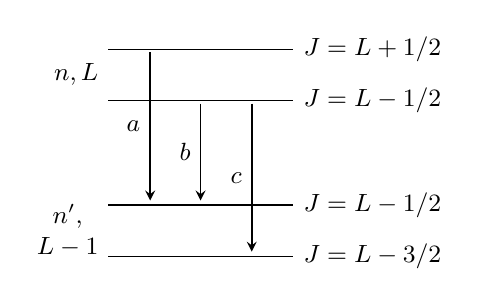
\begin{tikzpicture}[x=1cm,y=1cm,>=stealth,line width=.6pt,font=\small]
  \draw (-1.25,2.70)--(1.10,2.70);
  \draw (-1.25,2.05)--(1.10,2.05);
  \draw (-1.25,.72)--(1.10,.72);
  \draw (-1.25,.07)--(1.10,.07);
  \node[left] at (-1.25,2.38) {$n,L$};
  \node[left,align=center] at (-1.25,.40) {$n',$\\$L-1$};
  \node[right] at (1.10,2.70) {$J=L+1/2$};
  \node[right] at (1.10,2.05) {$J=L-1/2$};
  \node[right] at (1.10,.72) {$J=L-1/2$};
  \node[right] at (1.10,.07) {$J=L-3/2$};
  \draw[->] (-.72,2.66)--(-.72,.78) node[midway,left] {$a$};
  \draw[->] (-.08,2.01)--(-.08,.78) node[midway,left] {$b$};
  \draw[->] (.57,2.01)--(.57,.13) node[midway,left] {$c$};
\end{tikzpicture}

Fig.~1
\end{center}

Their relative intensities, denoted by $a$, $b$, and $c$, are more easily obtained from the rules (49.16) than directly from formula (49.15). Taking ratios of the total intensities of lines with one or the other common initial (or final) level gives two equations:
\[
\frac{b+c}{a}=\frac{2L}{2L+2},
\qquad
\frac{a+b}{c}=\frac{2L}{2L-2},
\]
and hence
\[
a:b:c=[(L+1)(2L-1)]:1:[(L-1)(2L+1)].
\]
For $L=1$, the lower level is not split, line $c$ is absent, and $a/b=2$.
